\chapter{Introduzione e Protocollo}
\section{Protocollo di consenso}
In una rete blockchain pubblica, nessuna singola entità detiene esclusivamente l'autorità di verificare e validare le transazioni, in quanto un avversario potrebbe falsificare una catena di blocchi con transazioni false e propagare la blockchain fasulla nella rete. 
Pertanto, un componente fondamentale delle reti blockchain è il protocollo di consenso, che consiste in un insieme di regole e procedure utilizzate per raggiungere un accordo comune, tra tutti i nodi partecipanti alla rete, sullo stato della blockchain.

\subsection{Proof Of Work (PoW)}
Uno dei protocolli di consenso più utilizzati è il Proof-of-Work (PoW) che si basa sul dimostrare di aver svolto uno sforzo computazionale per creare un blocco che soddisfa il protocollo di consenso. 
Questo processo, che porta ad avere un nuovo blocco valido da inserire nella blockchain, prende il nome di \textit{mining}.
In base alla blockchain considerata, il minatore che ha inserito il blocco può raccogliere le ricompense predefinite e/o le commissioni delle transazione contenute in tale blocco.

L'idea iniziale era che ogni partecipante potesse unirsi al processo di mining utilizzando le proprie risorse computazionali. 
In questo modo, un avversario per violare il protocollo PoW, deve necessariamente possedere una potenza di calcolo superiore a quella aggregata di tutti gli altri partecipanti al mining (attacco del 51\%). 
Tuttavia, questa minaccia inizia a diventare sempre più reale a causa della diffusione di miner basati su circuiti integrati specifici. 


\section{Mining: CPU vs GPU vs FPGA vs ASIC}
Tra le tecnologie maggiormente usate per il mining possiamo distinguere: ASIC (Application-Specific Integrated Circuits), FPGA (Field-Programmable Gate Arrays), GPU (Graphics Processing Units), e CPU (Central Processing Units). 

Ognuna di queste tecnologie viene impiegata per scopi precisi e presenta delle limitazioni rispetto alle altre.
Pertanto, dato che scegliere l'una piuttosto che l'altra comporta differenze in termini di efficienza e costi, è importante avere un'idea generale delle loro differenze.

\begin{itemize}
    \item Le \textbf{CPU}, le "generaliste del gruppo" presenti in ogni personal computer, offrono grande flessibilità, in quanto sono in grado di gestire un'ampia gamma di compiti a scapito dell'efficienza specializzata riscontrabile nelle altre tecnologie.
    \item Le \textbf{GPU}, inizialmente sviluppate per il rendering grafico, hanno trovato applicazioni diverse grazie alla loro capacità di elaborazione parallela, dimostrandosi strumenti potenti nei calcoli ad alta intensità di dati.
\end{itemize}

Nel contesto del mining di criptovalute, CPU e GPU sono state le prime scelte, ma con l'aumento della "concorrenza", ASIC e FPGA come soluzioni più efficienti.

\begin{itemize}
    \item Gli \textbf{FPGA (\textit{Field Programmable Gate Arrays})} possono implementare una vasta gamma di funzioni circuitali, in quanto sono fondamentalmente dispositivi modificabili fisicamente per creare lo specifico circuito elettronico che si desidera. 

    Poiché devono essere versatili, i componenti presenti internamente hanno molte caratteristiche che non vengono sfruttate. 
    Di conseguenza, nonostante possano raggiungere prestazioni superiori ad un computer general purpose, non sono ottimizzati per il consumo energetico e la velocità in un'applicazione specifica come quella del mining. 

    \item Un \textbf{ASIC (\textit{Application-specific integrated circuit})} è simile ad un FPGA in quanto utilizza un circuito elettronico cablato per eseguire una funzione computazionale. 
    A differenza di un FPGA, un ASIC può essere ottimizzato per il consumo energetico ridotto, la velocità o una combinazione di entrambi, comportandosi quindi sempre meglio di un FPGA programmato per fare lo stesso lavoro. 
    
    Gli svantaggi di un ASIC sono il costo di ingresso elevato ed il complesso processo di progettazione necessario per il loro sviluppo.

    La non modificabilità degli ASIC è il loro punto di forza in termini di consumo energetico e velocità, ma è anche una loro criticità. 
    Essendo progettati per eseguire un compito specifico, non possono essere adattati o aggiornati per eseguire funzioni diverse da quelle per cui sono stati progettati. 
    Pertanto, se una blockchain dovesse cambiare l'algoritmo di mining, gli ASIC progettati per minare su essa, diventerebbero obsoleti ed inefficaci poiché non modificabili.
\end{itemize}

Nonostante quest'ultima problematica, gli ASIC restano la minaccia più grande alle blockchain, in quanto offrono prestazioni superiori e un consumo energetico ottimizzato specificamente per il mining. 
Con il predominio di questi circuiti integrati, appositamente progettati per il calcolo di specifici PoW, la decentralizzazione delle reti blockchain e la loro integrità è messa a rischio. 



\subsubsection{Caso Bitcoin}
Osservando il grafico in Figura \ref{fig:btc-hashrate}, si può vedere come l'hashrate aggregato della rete Bitcoin, ovvero il numero di hash che vengono prodotti globalmente al secondo, è aumentato drammaticamente.

\begin{figure}[h!]
    \centering
    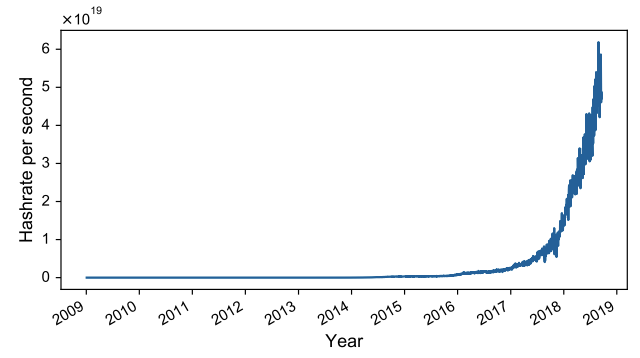
\includegraphics[width=0.55\linewidth]{images/bitcoin_hashrate.png}
    \caption{Hashrate della blockchain Bitcoin \cite{asic1}}
    \label{fig:btc-hashrate}
\end{figure}

La motivazione riconducibile a ciò è proprio l'avvento degli ASIC e la loro partecipazione al mining di Bitcoin.

Il mining basato su ASIC ha creato un picco barriera all'ingresso per il grande pubblico perché, chi interessato a minare, dovrebbe investire in attrezzature speciali per partecipare a tale processo.
A causa di ciò, come precedentemente accennato, le poche entità in grado di investire e mantenere un grande volume di ASIC potrebbero assumere il controllo della rete.
Pertanto, il mining basato su ASIC è maggiore vulnerabile all'attacco del 51\%. 

Ad esempio, partire da settembre 2018, i mining-pool\footnote{\textbf{Mining-pool}: minatori di criptovalute che uniscono le loro risorse per estrarre criptovalute e aumentare le probabilità di ottenere la ricompensa di un blocco} Bitcoin BTC.com e Antpool, che sono gestiti dalla stessa azienda che produce gli ASIC per la blockchain bitcoin, rappresentano oltre il 30\% del potere (hashrate) nella rete Bitcoin. 

Bitcoin crea quindi delle condizioni favorevoli per un ampio divario nel potere di voto tra partecipanti, 
violando il principio di \textit{un processore, un voto}, che Satoshi Nakamoto ha descritto nel whitepaper.
I proprietari di GPU e ASIC hanno infatti molto più potere di voto rispetto a coloro che utilizzano solo CPU.